\subsection{Long Short-Term Memory}
Long Short-Term Memory (LSTM) networks, introduced by Hochreiter and Schmidhuber (1997) \cite{hochreiter1997}, stand as a prominent advancement in the field of recurrent neural networks (RNNs). Unlike traditional RNNs, LSTMs possess the ability to effectively learn and utilize long-term dependencies within sequential data, overcoming the vanishing gradient problem that plagued earlier architectures. This section delves into the core principles of LSTMs, exploring their unique structure and the mechanisms that govern their memory capabilities.\\
While sharing the recurring chain-like structure of conventional RNNs, LSTMs differ significantly in the composition of their recurring modules. Instead of a single tanh layer, LSTMs employ four interconnected layers that interact in a coordinated fashion. As depicted in Figure \ref{fig:lstm-det}, information flows through the network via complete vectors, carried along by lines connecting the output of one node to the inputs of others. Pointwise operations, represented by pink circles, are performed on these vectors, and yellow boxes signify the learned neural network layers. Merging lines denote concatenation while forking lines indicate the copying of content to different locations within the network.\\
The key element of an LSTM lies in its cell state, symbolized by the horizontal line traversing the top of Figure \ref{fig:lstm-horz}. This cell state acts as a conveyor belt, continuously carrying information vertically across the network. Its inherent linearity facilitates the smooth and efficient flow of information, minimizing decay or distortion over time.\\
\begin{figure} [h]
    \centering
    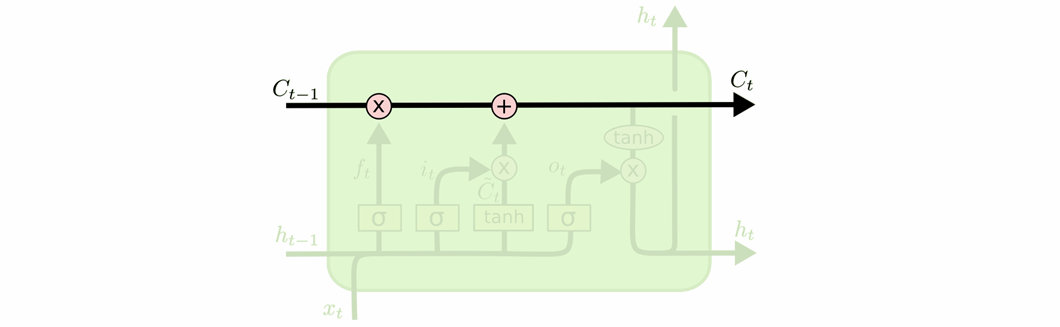
\includegraphics[width=0.75\linewidth]{images/dl/lstm-horz.png}
    \caption{Horizontal connection of cell state in LSTM.}
    \label{fig:lstm-horz}
\end{figure}
LSTMs possess the remarkable ability to selectively add or remove information from the cell state, a process meticulously controlled by specialized components known as gates. These gates, depicted as yellow boxes with sigmoid activation functions and subsequent pointwise multiplication operations, effectively regulate the flow of information through the network. The sigmoid layer outputs values between 0 and 1, determining the degree to which each element is allowed to pass through. A value of 0 signifies complete blockage, while 1 grants unrestricted passage.
An LSTM employs three distinct gates to safeguard and manage the cell state:
\begin{itemize}
    \item \textbf{Forget Gate:} This gate determines which information from the previous cell state should be retained. By outputting values near 0 for irrelevant information and values close to 1 for relevant information, the forget gate effectively filters the cell state, discarding outdated or unnecessary data.
    \item \textbf{Input Gate:} This gate controls the flow of new information into the cell state. It considers both the current input and the previous hidden state, selectively adding relevant information to the cell state based on its output values.
    \item \textbf{Output Gate:} This gate regulates the information that is exposed to the rest of the network. By applying the sigmoid function to the current cell state and the previous hidden state, the output gate determines which portions of the cell state will contribute to the output of the LSTM unit.
\end{itemize}

\begin{figure} [h]
    \centering
    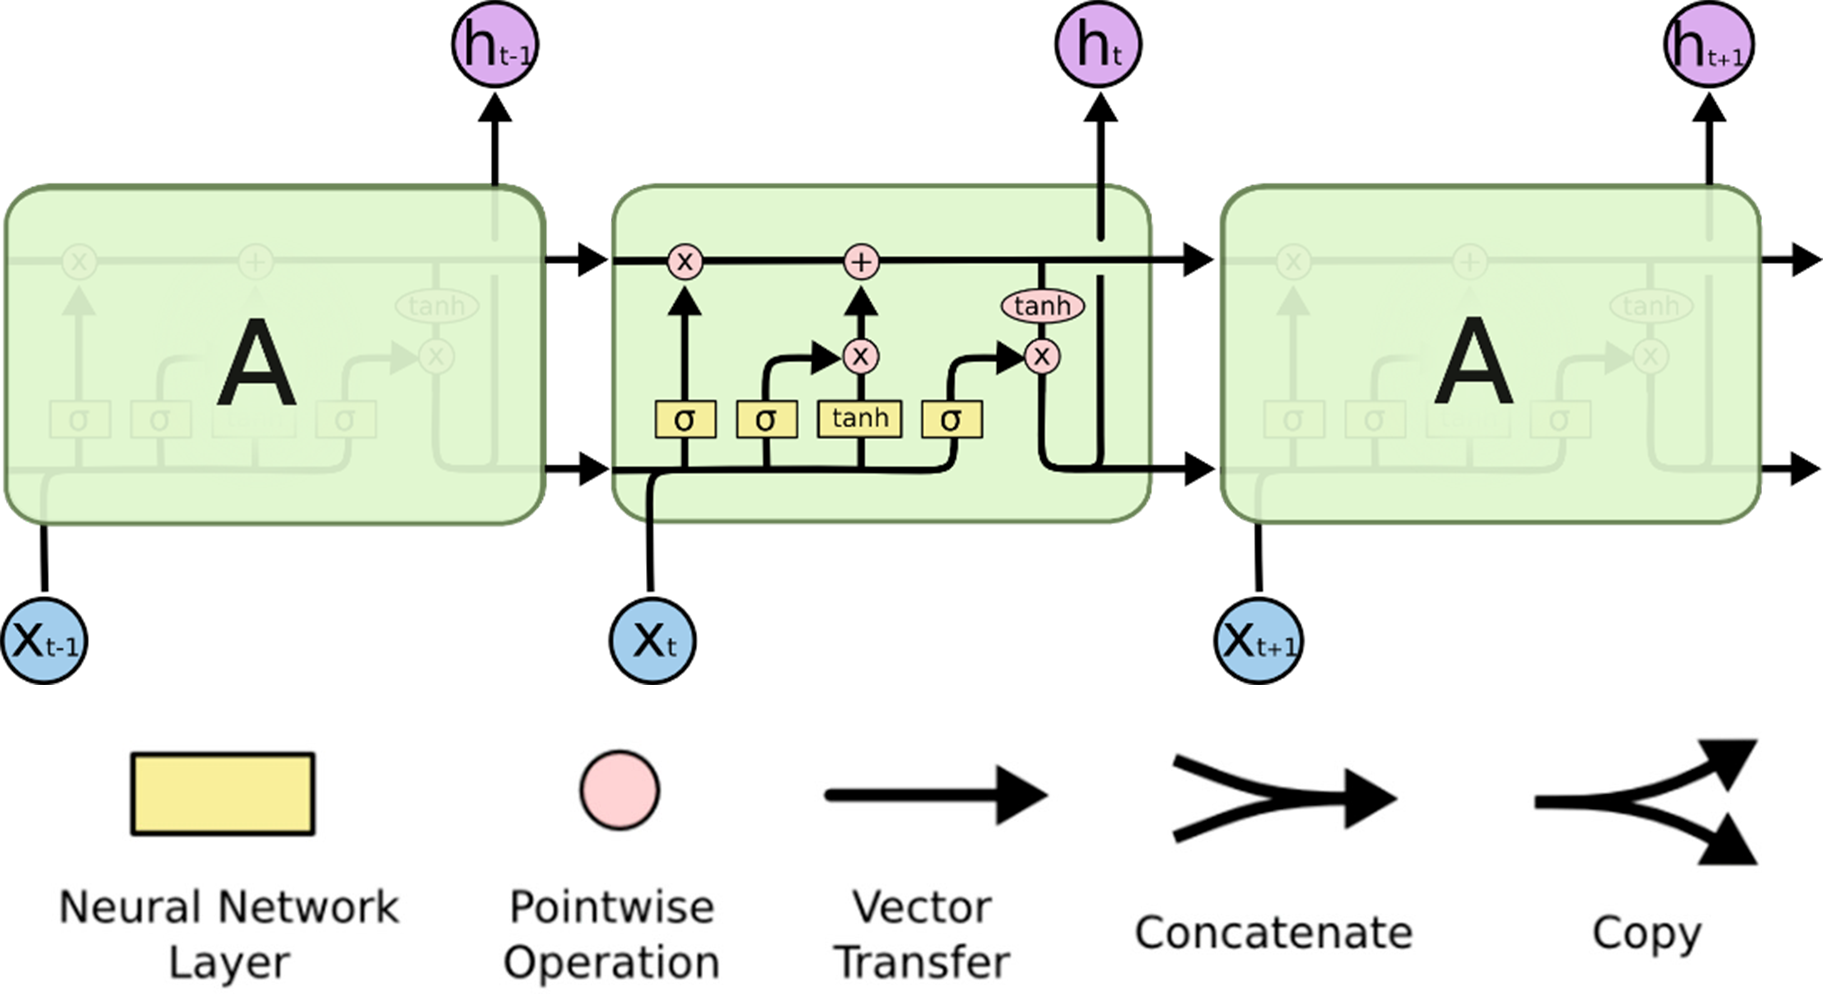
\includegraphics[width=0.75\linewidth]{images/dl/lstm-det.png}
    \caption{Information Flow in a LSTM. Each directed line in the graph corresponds to a complete vector, transmitting information from the output of one node (neuron) to the inputs of others. Pointwise operations, such as vector addition, are denoted by pink circles, while the yellow boxes represent trainable neural network layers. Merging lines indicate vector concatenation, where the elements of two or more vectors are combined to form a single longer vector. Conversely, a forking line signifies the content being copied, with identical copies directed to different locations within the network.}
    \label{fig:lstm-det}
\end{figure}

\subsubsection{LSTM's Internal Mechanism}
The first stage involves determining which information to discard from the previous cell state $C_{t-1}$. This critical decision is facilitated by a "forget gate" implemented as a sigmoid layer. This layer analyzes both the previous hidden state $h_{t-1}$ and the current input $x_t$ to generate a forget vector $f_t$ with values between 0 and 1 for each element of $C_{t-1}$ as illustrated in Equation \ref{eq:lstm-forget}. A $f_t$ value of 1 indicates complete retention, while 0 signifies absolute removal.
The following equation describes the forget gate's operation:
\begin{equation} \label{eq:lstm-forget}
    f_t = \sigma(W_f \cdot [h_{t-1}, x_t] + b_f)
\end{equation}
Consider an LSTM-based language model predicting the next word in a sentence. The cell state might hold information like subject gender for pronoun agreement. When encountering a new subject, the forget gate activates to discard the irrelevant gender information about the previous subject.\\
The second stage focuses on incorporating new information into the cell state. This process unfolds in two steps. First, an "input gate" sigmoid layer generates an update vector $i_t$ specifying which state elements require modification. Subsequently, a tanh layer creates a candidate update vector $\tilde{C}_t$ containing potential new values as shown in Equations \ref{eq:lstm-input} and \ref{eq:lstm-candidate}. These two vectors are then combined to form the state update.
The equations governing this stage are as follows:
\begin{equation} \label{eq:lstm-input}
    i_t = \sigma(W_i \cdot [h_{t-1}, x_t] + b_i)
\end{equation}
\begin{equation} \label{eq:lstm-candidate}
    \tilde{C}_t = tanh(W_C \cdot [h_{t-1}, x_t] + b_C)
\end{equation}
Here, the intent is to integrate the gender of the new subject into the cell state, replacing the discarded information about the previous subject. The input gate determines which aspects of the state require an update (e.g., subject gender), while the tanh layer generates potential new values for those elements.\\
The third stage bridges the gap between the old and the updated cell state $C_t$. Building upon the decisions made in the previous stages, it implements the actual state update. First, Ct-1 is multiplied by ft, effectively discarding the elements marked for removal by the forget gate. Next, the scaled candidate update vector $i_t * \tilde{C}_t$ is added to the filtered Ct-1, resulting in the new cell state $C_t$.\\
This stage witnesses the actual removal of old subject gender information and the insertion of new information about the current subject's gender, as determined by the forget and input gates in the earlier steps.\\
While the cell state holds the complete processed information, the output undergoes a selective filtering process. An "output gate" sigmoid layer determines which cell state components are relevant for the current output. Subsequently, the tanh-transformed cell state is multiplied by the output gate vector, ensuring that only the chosen information is emitted.\\
After processing a subject, the model might want to output information relevant to the upcoming verb, such as its tense and agreement morphology. The output gate decides which aspects of the cell state (e.g., subject number) are crucial for predicting the verb and filters the output accordingly.\\
By meticulously managing the information flow within the cell state, LSTMs retain long-term dependencies while adapting to new information in sequential data, making them a powerful tool for various applications.

\subsubsection{Bidirectional LSTM}
Bidirectional LSTMs (BiLSTMs) are an extension of traditional LSTMs that can improve model performance on sequence classification problems. They work by processing the input sequence in both directions with two separate hidden layers which are then fed forwards to the same output layer.
The motivation behind BiLSTMs is that the output at time $t$ may not only depend on the previous elements in the sequence but also future elements. For example, to predict a missing word in a sequence you want to look at both the left and the right context.
The two separate hidden layers of a BiLSTM are typically referred to as the forward and backward layers. The forward layer passes over the sequence from left to right and the backward layer passes over the sequence from right to left. The outputs of these two layers are usually concatenated at each time step, although there are other options, e.g., summation.
The output of a BiLSTM at time $t$ is a concatenation of the forward hidden state $h_t^f$ and the backward hidden state $h_t^b$:
\begin{equation}
    h_t = [h_t^f, h_t^b]
\end{equation}
where $h_t^f$ is the hidden state of the forward layer at time $t$ and $h_t^b$ is the hidden state of the backward layer at time $t$. This bidirectional configuration allows the model to effectively "anticipate" future information by starting from the end of a sequence, such as an audio clip.
\begin{figure} [h]
    \centering
    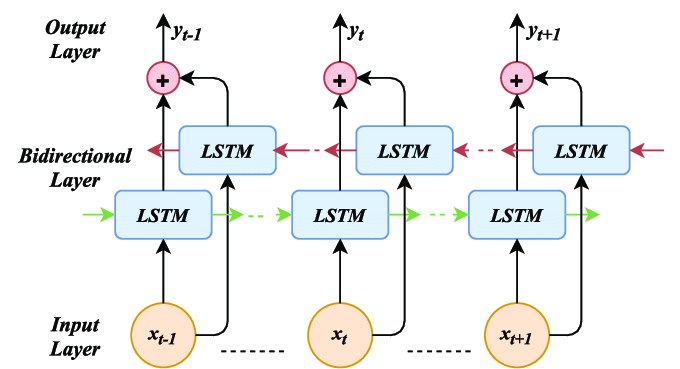
\includegraphics[width=0.75\linewidth]{images/dl/bilstm.png}
    \caption{Bidirectional LSTM model showing the input and output layers. The red arrows represent the backward sequence track and the green is the forward sequence track.}
    \label{fig:lstm-bi}
\end{figure}

